% chapter5.tex
% Muon events, threshold analysis
Analysis of LED events can only be applied on the four extra top modules. To determine the stability of the total \mvs, aging of all modules are investigated. In this chapter, the muon-events are selected and analysed. The change of the detection efficiency of each module are calculated.

\section{Analysis of muon events}


\begin{itemize}
  \item selection criteria, runs...
  \item Landau-spectrum, method detailed for M6..,  compare M8 with LED.
\end{itemize}

\subsection{Selection of muon-veto data}
All the data from Run70 (Aug 2010) to Run138 (Mar 2017) are investigated in the following analysis. First, data taken when the \mvs{} was not fully closed are cut. As described in \ref{sec:muon-setup}, two lasers measure the position of the upper part of the muon-veto every 15 minutes. Time periods when the gap size deviates more than 5 cm from the closed configuration are cut, since the \mvs{} is either fully closed or fully opened. When the system is opened, the detection efficiency of through-going muons decreases and the background rate increases largely.

When the \mvs{} is closed, most muons go through at least 2 modules. Therefore a coincidence in 2 distinct modules is required for selecting muon events. An energy deposit with full information in each module is required--i.e.\ both TDCs and ADCs have non-zero values. It respectively reduces events caused by secondary particles or natural backgrounds since they mostly deposit less energy than muons. By applying this cut criterium, the event rate in one module is reduced to the order of $\SI{10}{events/day}$.

\subsection{Data analysis}
As mentioned in section \ref{sec:muon-working}, the spectrum of muon energy deposit in modules can be described by a Landau distribution. The ADC values of muon events in a time period are fitted with a Landau distribution and the obtained MPVs in different time periods are used to analyse the long term behaviour of the \mvs. The fig.\ \ref{fig:Landau_M6} shows an example of the Landau fit. Since the muon event rate is low, the obtained ADC values in a two months period are combined to perform each fit.

\begin{figure}[ht]
  \centering
  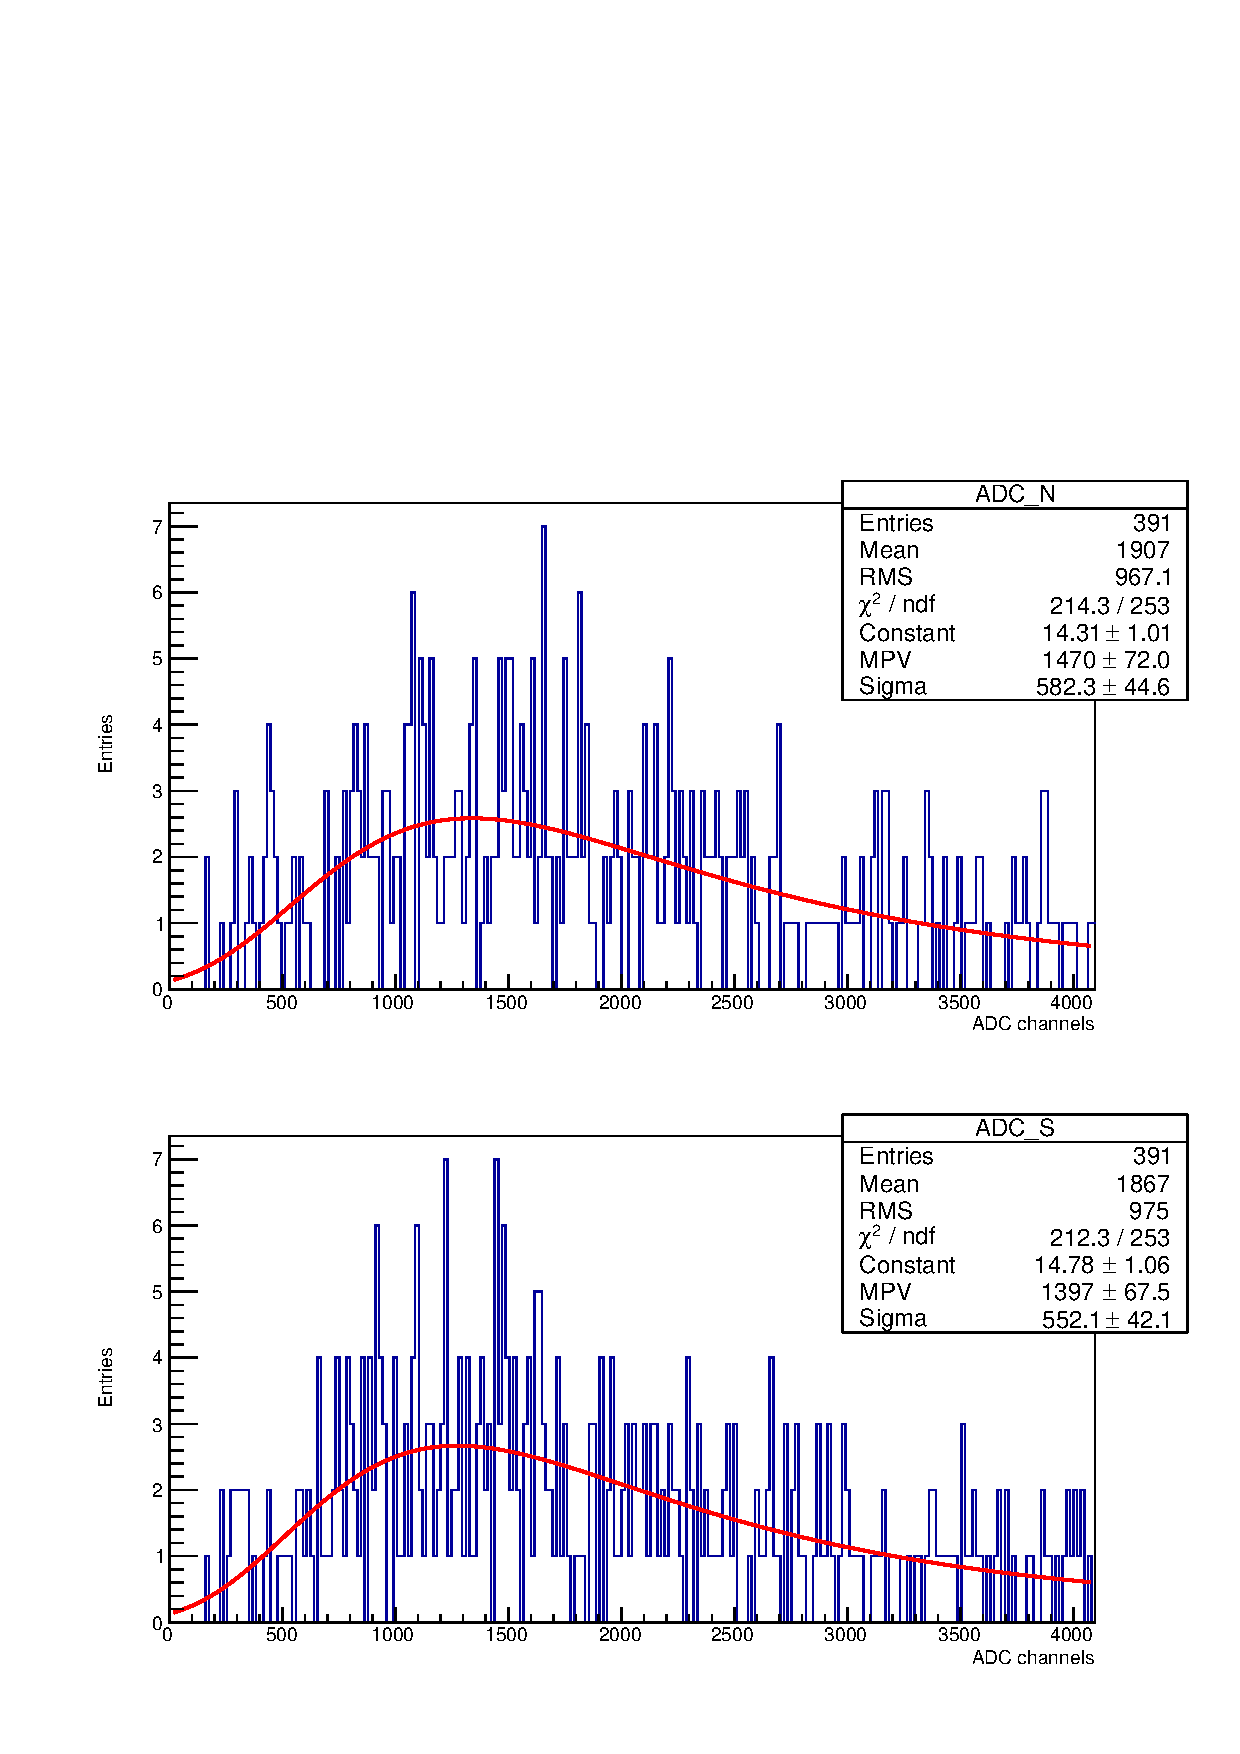
\includegraphics[width=0.5\textwidth{}]{./fig/LandauFitM6.pdf}
  \caption{Example of a Landau spectrum fit in M6. The fit uses a log likelihood method in ROOT.}
  \label{fig:Landau_M6}
\end{figure}

The MPVs obtained from the Landau fit are plotted over time (see fig.\ \ref{fig:MPV}). It is to be noticed that the data points have rather large uncertainty, which is partially due to the smeared spectrum. As mentioned before, the light output is strongly position dependent and decreases exponentially with the path length from the interaction point to the PMT group. Furthermore, there are some sudden changes of the MPVs. The reason could be the restart of the \mvs{} after operations.
Despite the various effects, the MPVs have a clear decrease of about $\SI{500}{channels}$ over the past few years.

The change of the MPVs are again approximated by a linear regression and the obtained slopes are listed in tab.\ \ref{tab:mpv}.

The value obtained in M8 is also listed for comparison with the result from LED events. The decrease of the  is

The abnormal increase of ADC mean values of LED S in M8 (see tab.\ref{tab:led}) is not to be found in the data obtained from muon events. Therefore it can be concluded that the problem is merely due to the behaviour of the LED but not the scintillator module.


\begin{figure}[htb]
  \centering
  \begin{subfigure}{0.55\linewidth}
    \centering
    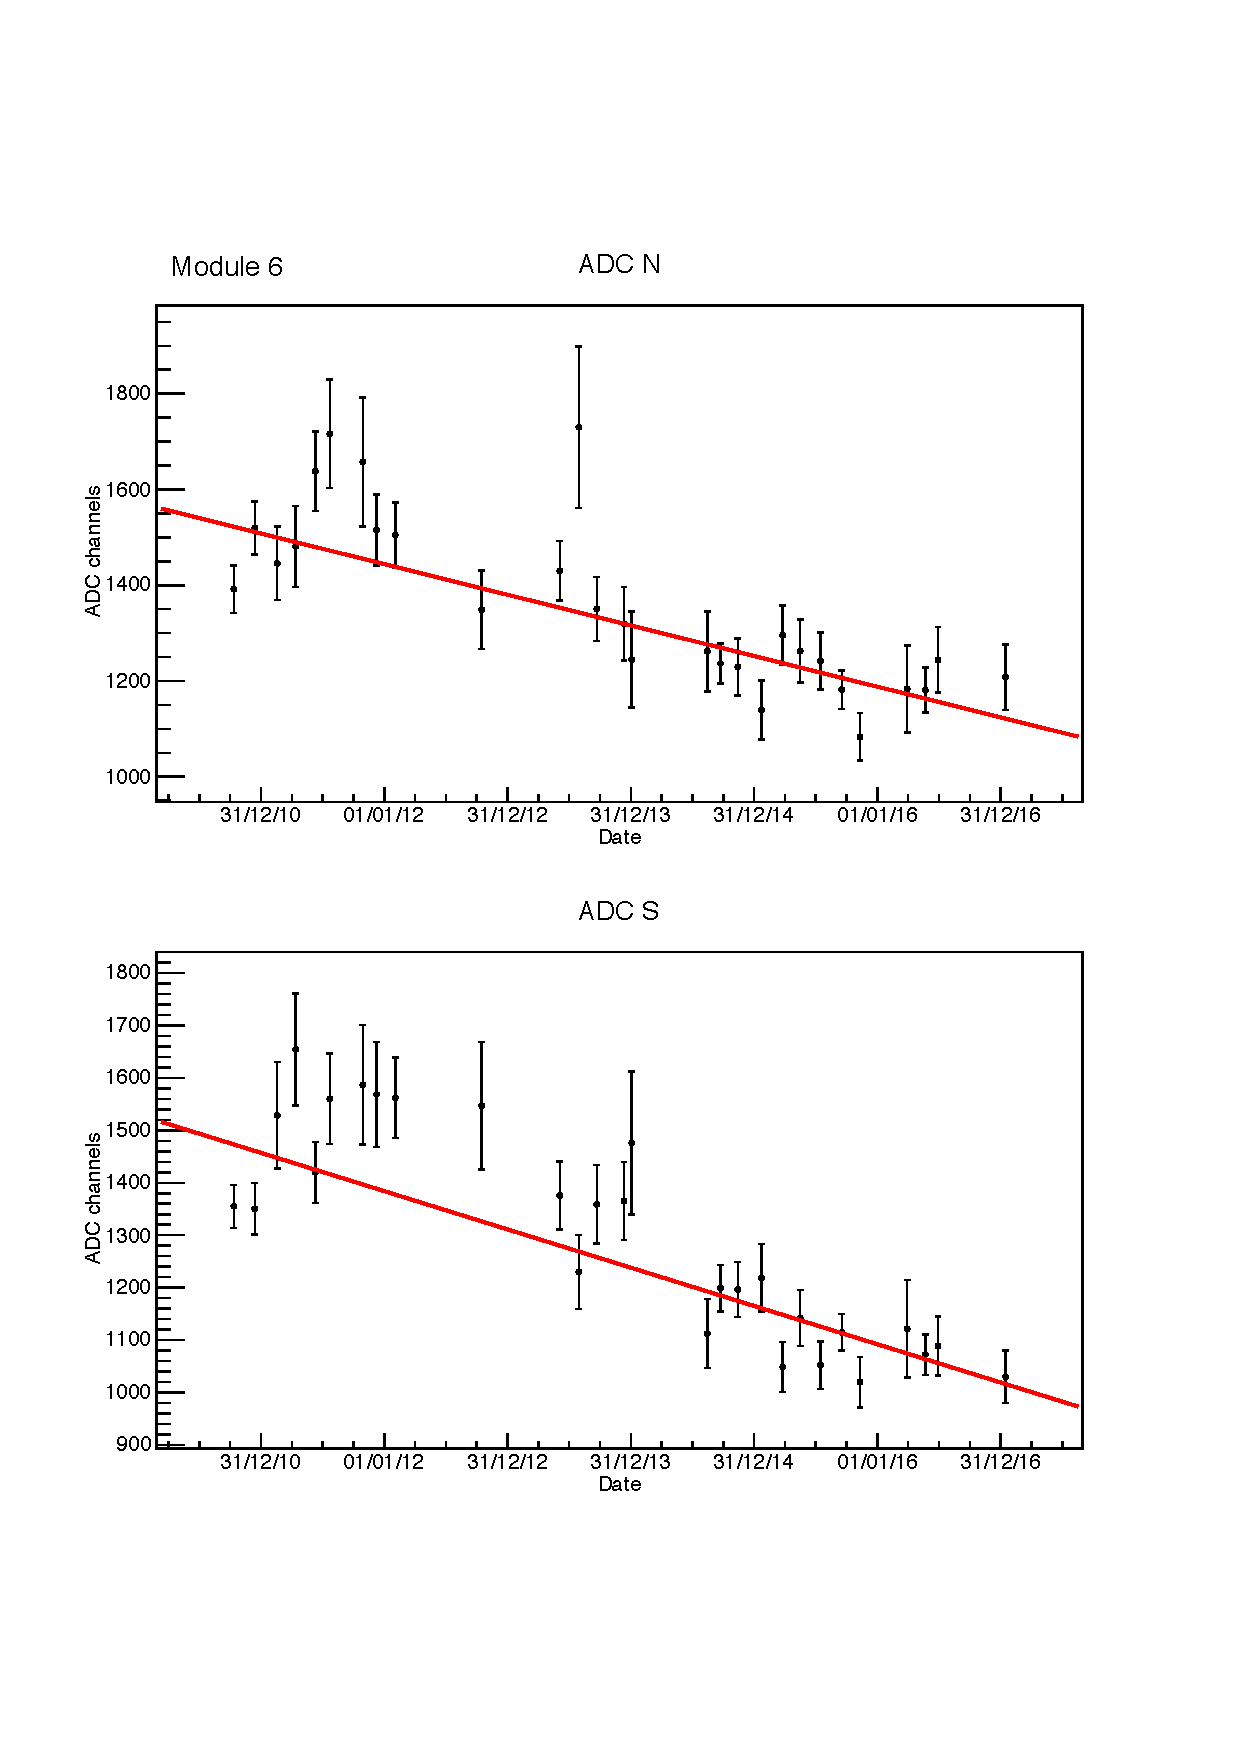
\includegraphics[width=\linewidth{}]{./fig/M6mpv.pdf}
    \caption{}
    \label{fig:MPV_M6}
  \end{subfigure}
  \begin{subfigure}{0.55\linewidth}
    \centering
    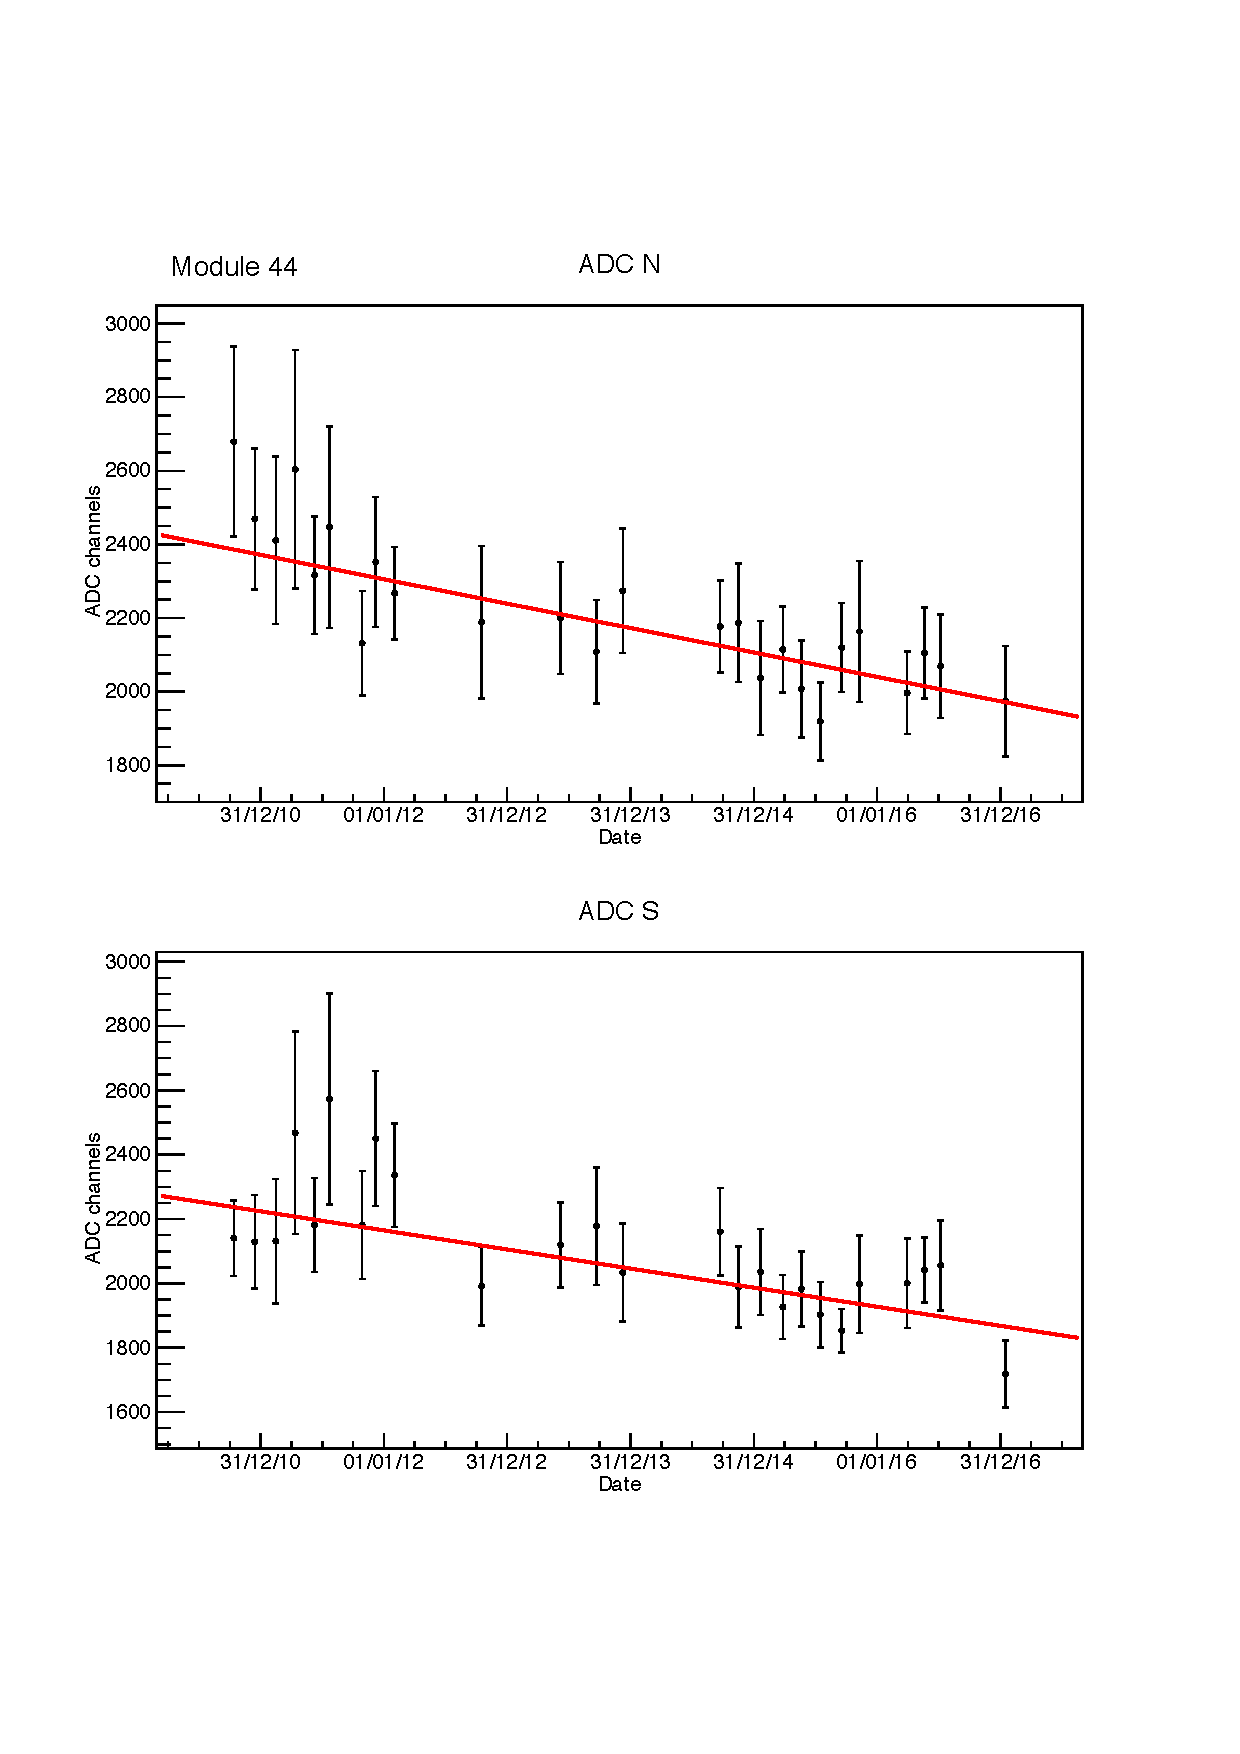
\includegraphics[width=\linewidth{}]{./fig/M44mpv.pdf}
    \caption{}
    \label{fig:MPV_M44}
  \end{subfigure}
  \caption{MPVs over time with linear fits in two example modules. The two upper figures show the MPVs in M6 (top module) and the two lower figures show the MPVs in M44 (bottom module).}
  \label{fig:MPV}
\end{figure}
%
%\begin{figure}[htb]
%  \centering
%  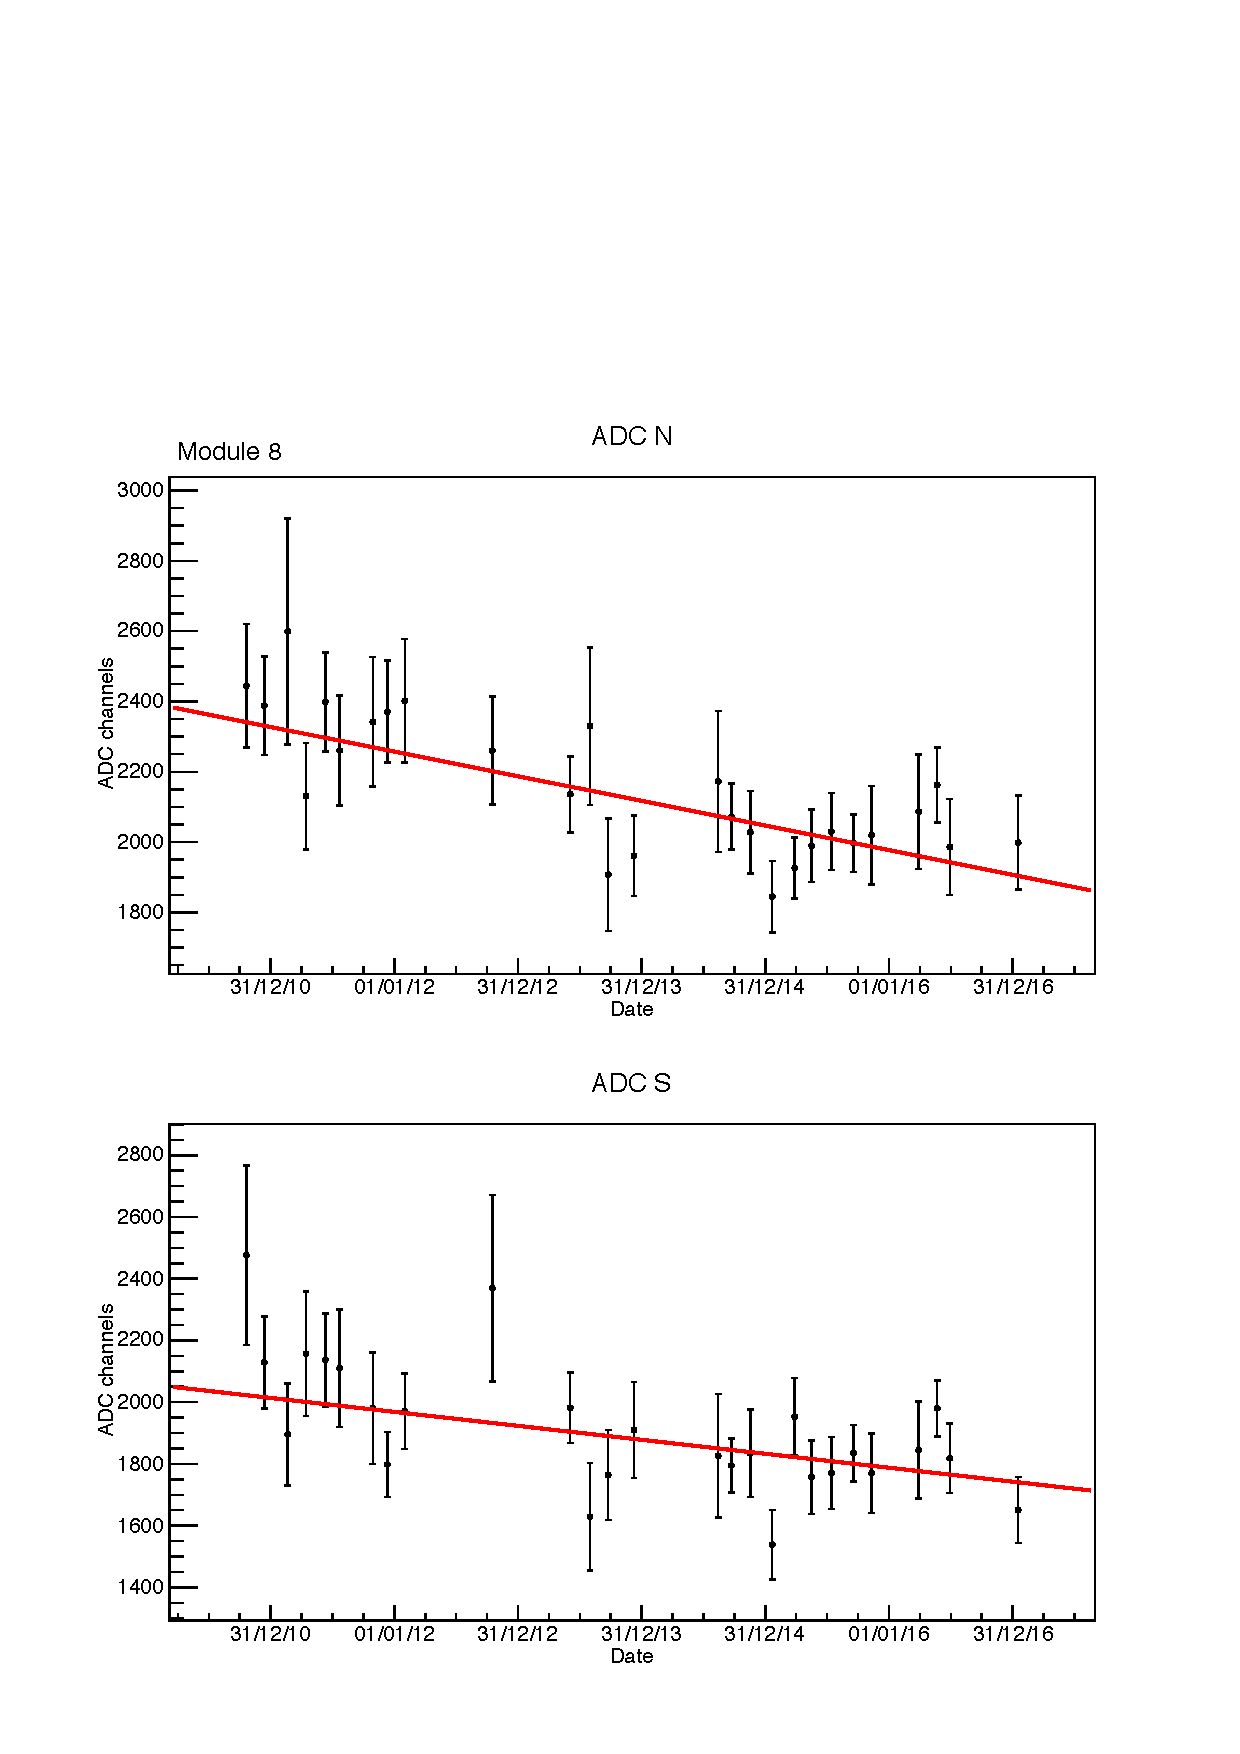
\includegraphics[width=0.6\textwidth{}]{./fig/M8mpv.pdf}
%  \caption{MPVs over time with linear fit in M8.}
%  \label{fig:Landau_M8}
%\end{figure}

\begin{table}[hb]
  \centering
  \caption{Slopes of the linear regressions of MPVs in example modules M6, M8 and M44. The statistical uncertainty is obtained from the fit program in ROOT. }
  \label{tab:mpv}
  \begin{tabular}{c c c c}
  \toprule
        & \multicolumn{2}{c}{slope in channels/month} \\
        & ADC N & ADC S \\
  \midrule
  M6  & $-5.44\pm1.34$ & $-4.87\pm1.12$ \\
  M8  & $-5.26\pm0.52$ & $-6.00\pm0.46$ \\
  M44 & $-5.76\pm3.71$ & $-3.71\pm1.12$ \\
  \bottomrule
  \end{tabular}
\end{table}




\section{Determination of the detection efficiency}


\begin{itemize}
  \item conversion threshold,effective threshold
  \item method to determine threshold
  \item result, change of efficiency
\end{itemize}

\begin{figure}[ht]
  \centering
  \begin{subfigure}{0.7\linewidth}
    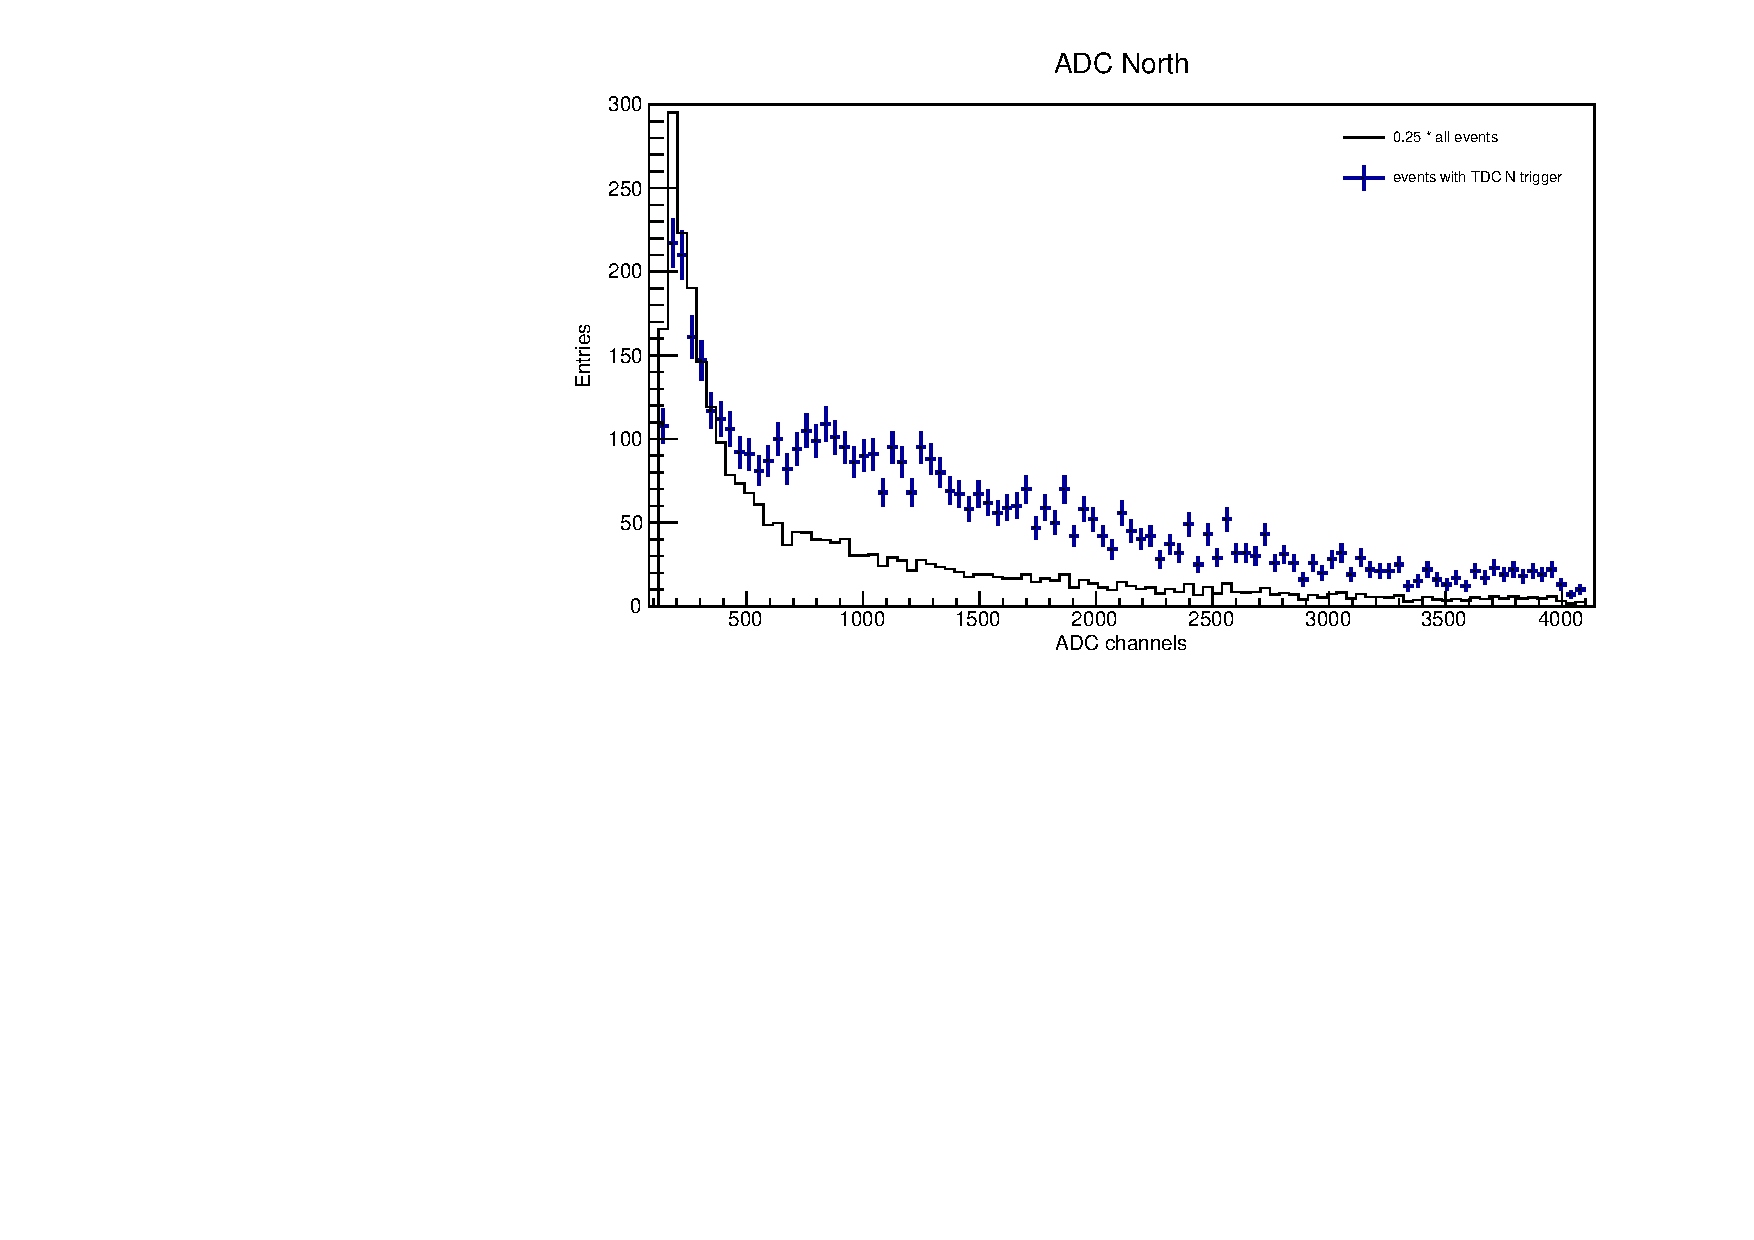
\includegraphics[width=\linewidth{}]{./fig/M6AdcNorth2Histo.pdf}
    \caption{Example of the spectrum with and without trigger condition of ADC N in M6. The blue data points are events which satisfy the trigger condition in the same end (Northern PMT group). The spectrum of all events (black) are scaled by a factor of 4.}
    \label{fig:2HistoM6}
  \end{subfigure}
  \begin{subfigure}{0.7\linewidth}
    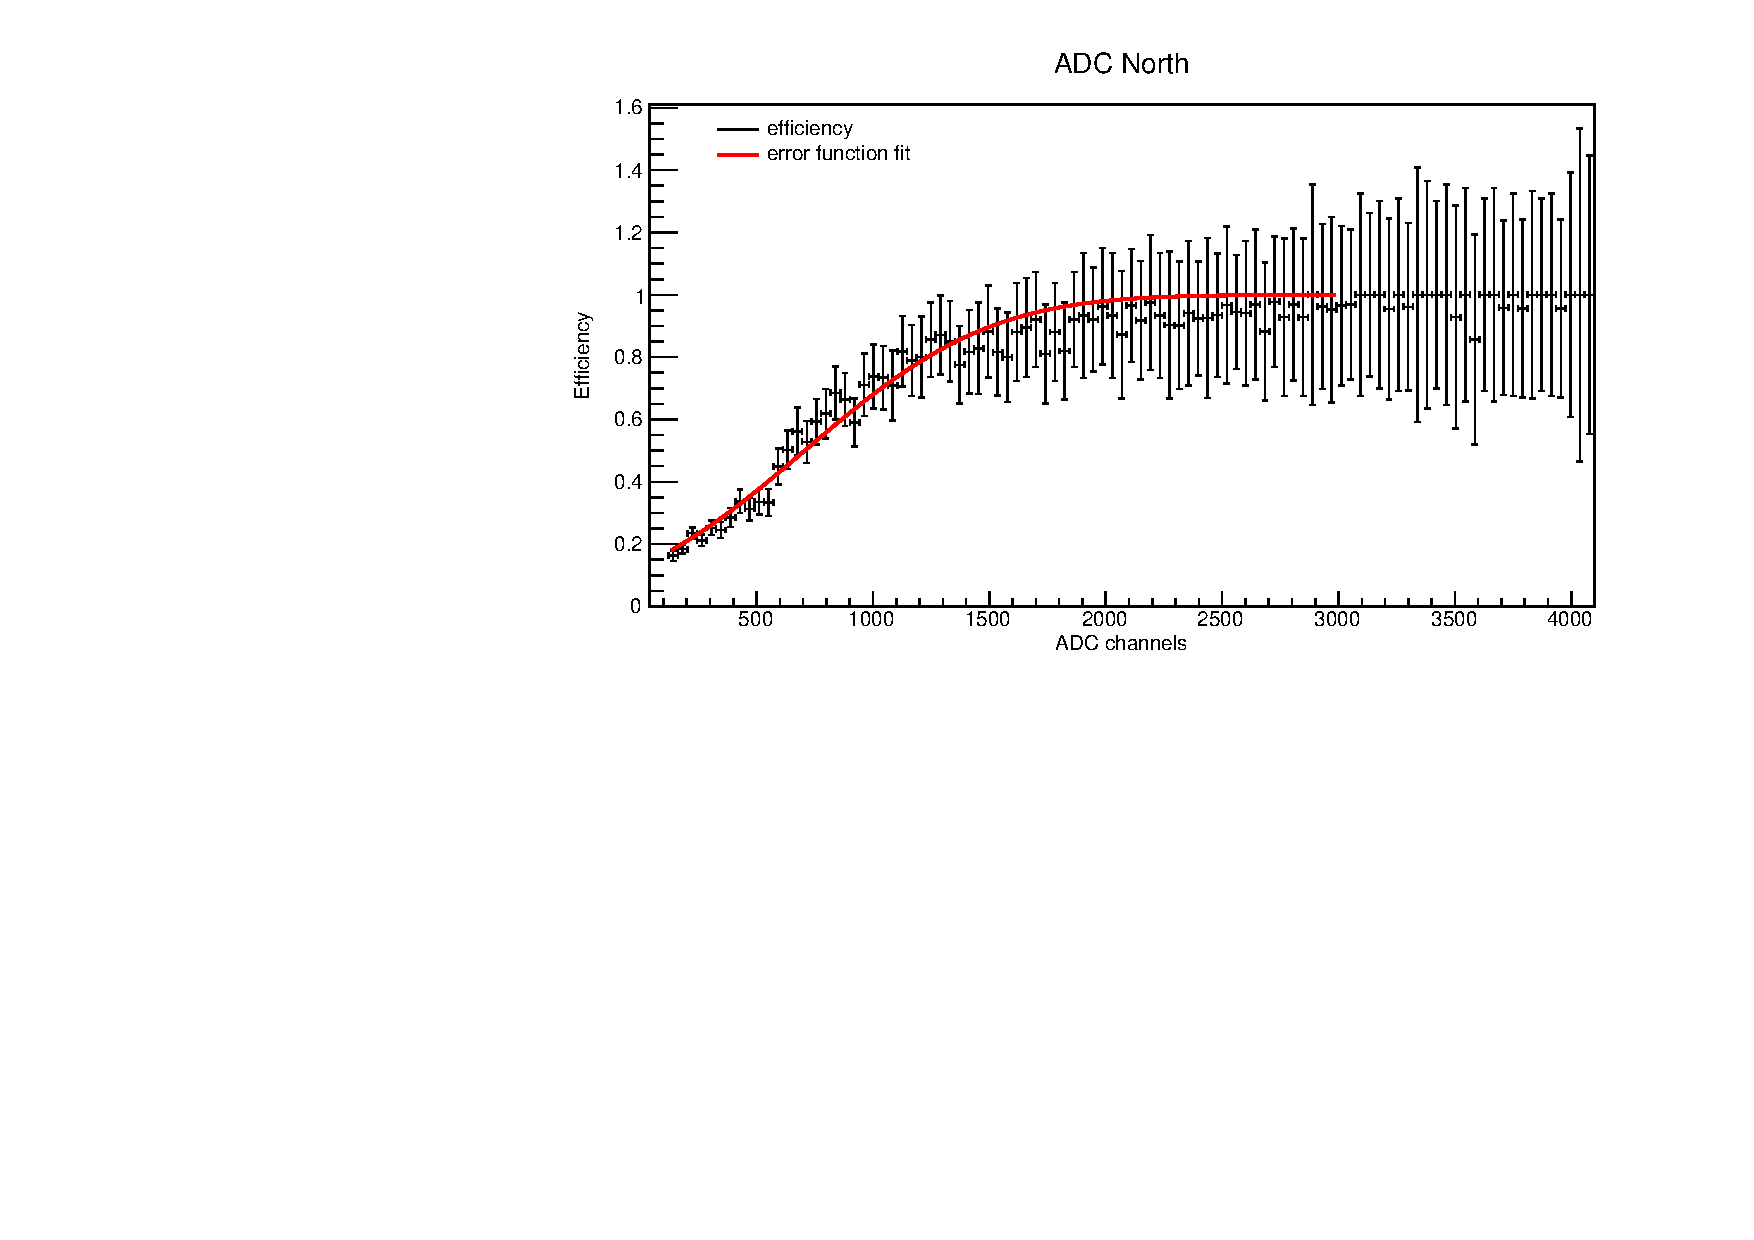
\includegraphics[width=\linewidth{}]{./fig/M6AdcNortheff_late.pdf}
    \caption{}
    \label{fig:eff_lateM6}
  \end{subfigure}
\end{figure}

\begin{figure}[ht]
  \centering
  \begin{subfigure}{0.7\linewidth}
    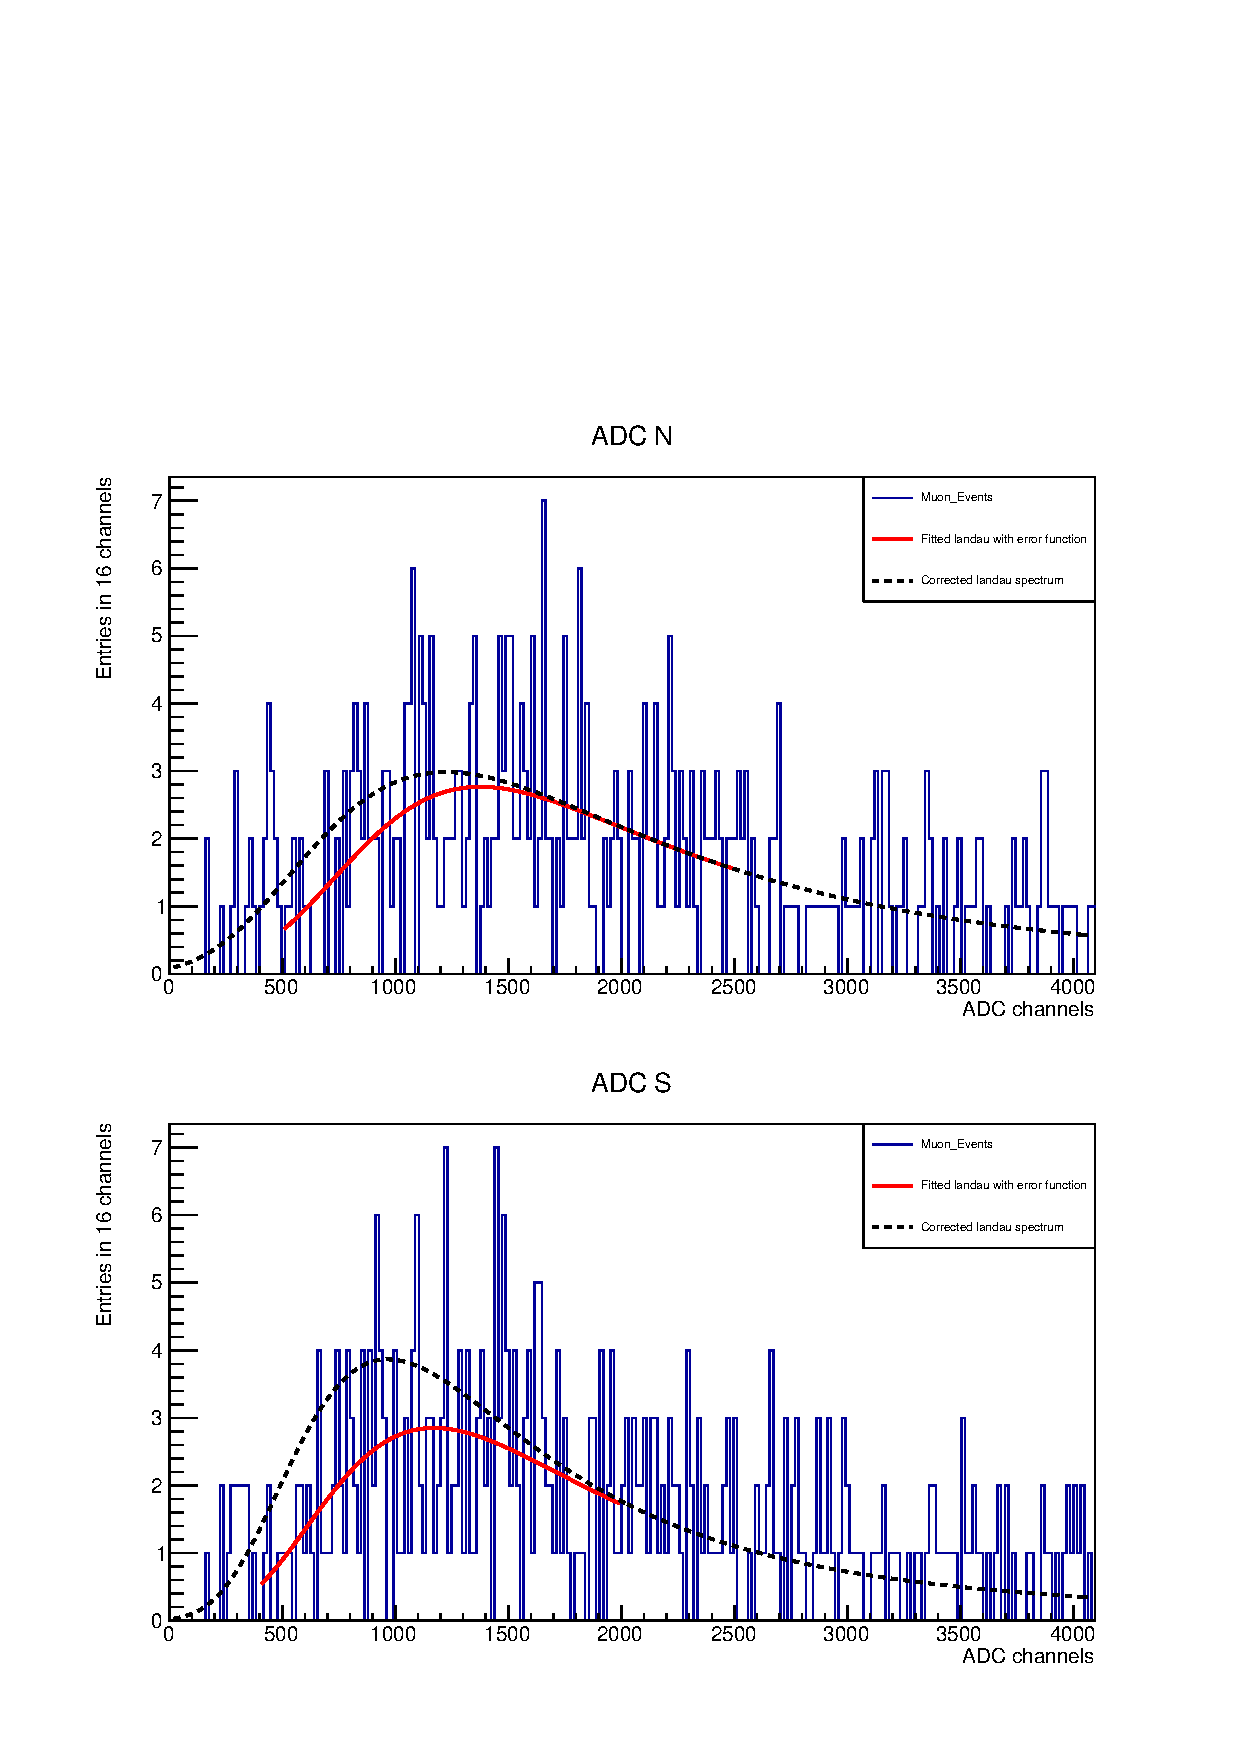
\includegraphics[width=\linewidth{}]{./fig/70M6CorrectedLandau.pdf}
    \caption{}
    \label{fig:2HistoM6}
  \end{subfigure}
  \begin{subfigure}{0.7\linewidth}
    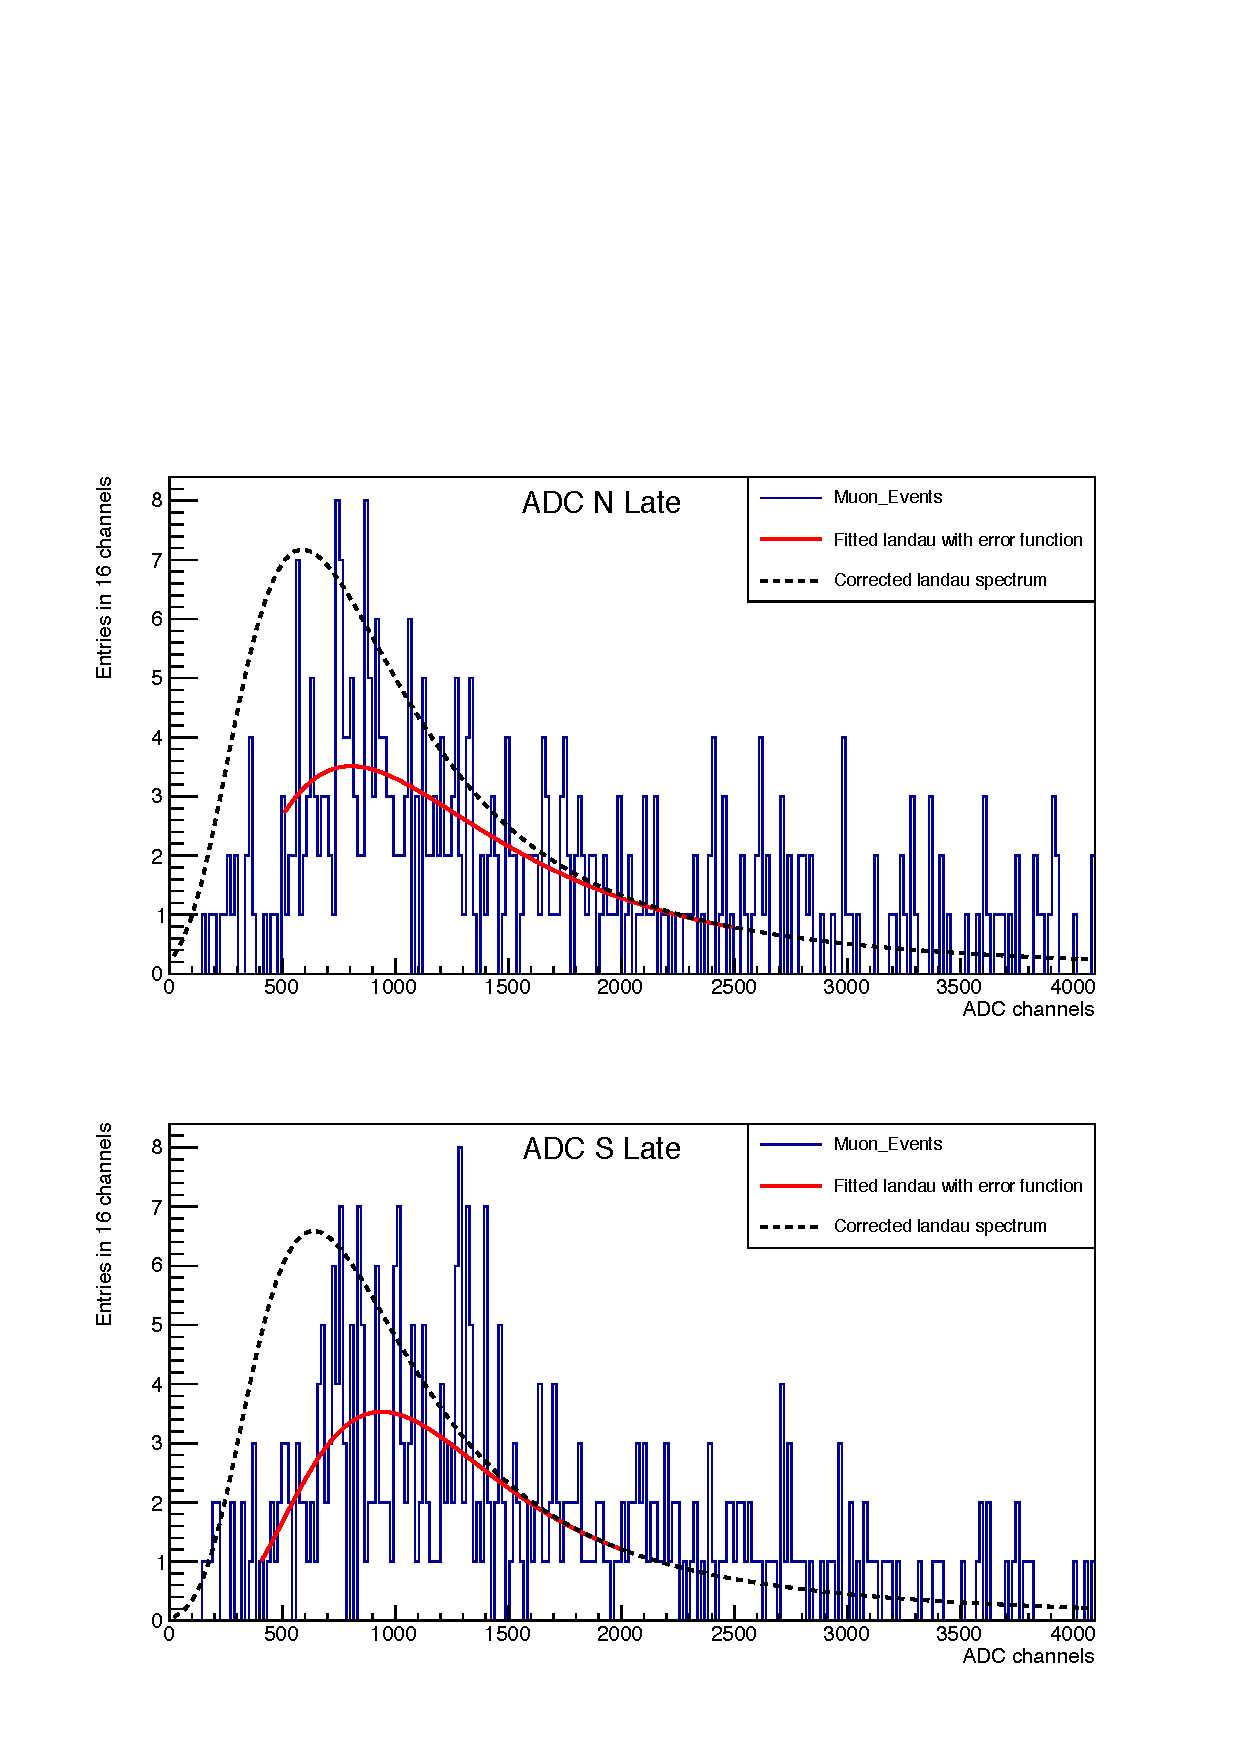
\includegraphics[width=\linewidth{}]{./fig/124M6CorrectedLandau.pdf}
    \caption{}
    \label{fig:eff_lateM6}
  \end{subfigure}
\end{figure}
